\usepackage[T1]{fontenc}
\usepackage[utf8]{inputenc}
\usepackage{stmaryrd}
\usepackage{setspace}
\usepackage{mathrsfs}
\usepackage[ngerman]{babel}
\usepackage{amssymb}
\usepackage{amsmath}
\usepackage{enumitem}
\usepackage[colorlinks,linkcolor=black]{hyperref} 
\usepackage{fancyhdr}
\usepackage{subcaption}
\usepackage{graphicx}
\usepackage{lipsum}
\usepackage{float}
\usepackage{color}
\usepackage{listings}


\usepackage{listings}
\usepackage{color}
\usepackage{hyperref}
\usepackage{longtable}
\hypersetup{
     colorlinks   = true,
     citecolor    = gray,
     linkcolor    = blue,
     urlcolor     = blue,
}

\definecolor{mygreen}{rgb}{0,0.6,0}
\definecolor{mygray}{rgb}{0.5,0.5,0.5}
\definecolor{mymauve}{rgb}{0.58,0,0.82}

\lstset{ %
  backgroundcolor=\color{white},   % choose the background color; you must add \usepackage{color} or \usepackage{xcolor}
  basicstyle=\small,        % the size of the fonts that are used for the code
  breakatwhitespace=false,         % sets if automatic breaks should only happen at whitespace
  breaklines=true,                 % sets automatic line breaking
  captionpos=b,                    % sets the caption-position to bottom
  commentstyle=\color{mygreen},    % comment style
  deletekeywords={...},            % if you want to delete keywords from the given language
  escapeinside={\%*}{*)},          % if you want to add LaTeX within your code
  extendedchars=true,              % lets you use non-ASCII characters; for 8-bits encodings only, does not work with UTF-8
  frame=single,	                   % adds a frame around the code
  keepspaces=true,                 % keeps spaces in text, useful for keeping indentation of code (possibly needs columns=flexible)
  keywordstyle=\color{blue},       % keyword style
  language=VHDL,                 % the language of the code
  otherkeywords={*,...},           % if you want to add more keywords to the set
  numbers=left,                    % where to put the line-numbers; possible values are (none, left, right)
  numbersep=5pt,                   % how far the line-numbers are from the code
  numberstyle=\tiny\color{mygray}, % the style that is used for the line-numbers
  rulecolor=\color{black},         % if not set, the frame-color may be changed on line-breaks within not-black text (e.g. comments (green here))
  showspaces=false,                % show spaces everywhere adding particular underscores; it overrides 'showstringspaces'
  showstringspaces=false,          % underline spaces within strings only
  showtabs=false,                  % show tabs within strings adding particular underscores
  stepnumber=1,                    % the step between two line-numbers. If it's 1, each line will be numbered
  stringstyle=\color{mymauve},     % string literal style
  tabsize=2,	                   % sets default tabsize to 2 spaces
  linewidth=15cm,
  title=\lstname                   % show the filename of files included with \lstinputlisting; also try caption instead of title
}

\usepackage{caption}
\captionsetup[lstlisting]{font={scriptsize}}
\DeclareGraphicsExtensions{.pdf,.png,.jpg}

\pagestyle{fancy}
\lfoot{Carl Schaffer}
\rfoot{carl.schaffer@cern.ch}
\cfoot{-\thepage-}
\renewcommand{\headrulewidth}{0.6pt}
\renewcommand{\footrulewidth}{0.6pt}
\setlength{\headheight}{37pt}
\setlength{\parindent}{0pt}
\renewcommand{\familydefault}{\sfdefault}

\newcommand{\exercise}[2]{\section{#1}\hfill{}\\}

\newcommand{\doublefig}[2]{\begin{center}
  \begin{tabular}{ll}
    a.) &b.)\\
    \includegraphics[width=.3\textwidth]{#1}&  \includegraphics[width=.3\textwidth]{#2} 
  \end{tabular}
\end{center}
}

\newcommand{\doublefignolabel}[2]{\begin{center}
  \begin{tabular}{ll}
    \includegraphics[width=.2\textwidth]{#1}&\includegraphics[width=.3\textwidth]{#2}
  \end{tabular}
\end{center}
}


\newcommand{\signal}[1]{\texttt{#1}}
\newcommand{\stdl}{\lstinline$standard_logic$}
\newcommand{\stdlv}[2]{\lstinline$standard_logic_vector(#1 downto #2)$}
\newcommand{\vhdl}[1]{\lstinline$#1$}
\newcommand{\loghi}{\vhdl{'1'}}
\newcommand{\loglo}{\vhdl{'0'}}

\newcommand*{\bashcode}{\lstinline[{language=[LaTeX]TeX}]}
\newcommand{\bash}[1]{\bashcode$#1$}
\newcommand{\git}{\texttt{GIT}}

\newcommand{\nandGate}{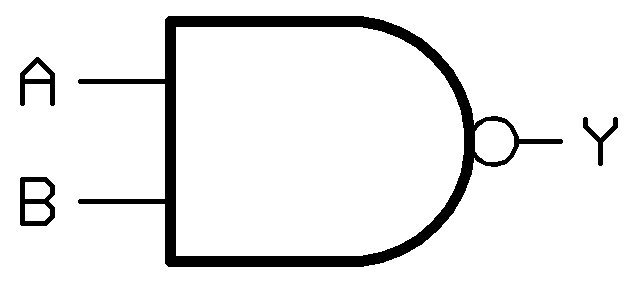
\includegraphics[width=3cm]{./images/nand}}
\newcommand{\andGate}{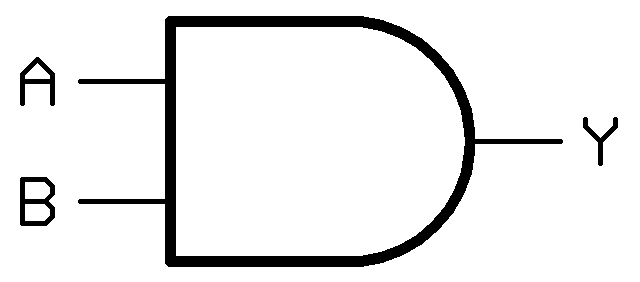
\includegraphics[width=3cm]{./images/and}}
\newcommand{\notGate}{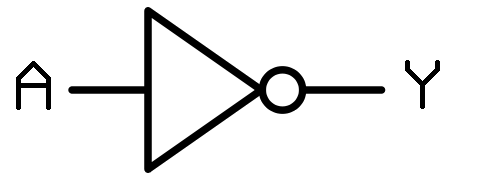
\includegraphics[width=3cm]{./images/not}}
\newcommand{\xorGate}{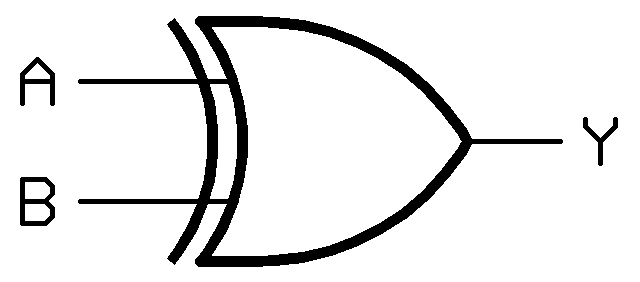
\includegraphics[width=3cm]{./images/xor}}
\newcommand{\orGate}{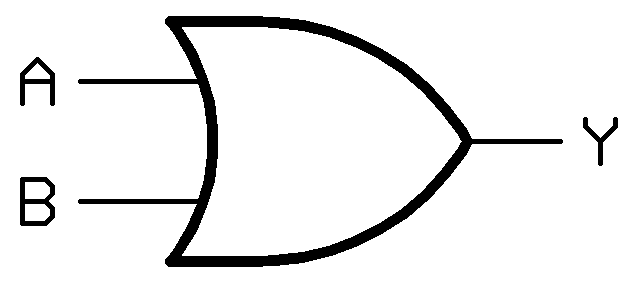
\includegraphics[width=3cm]{./images/or}}

\newcommand{\ise}{XILINX ISE}

\newcommand{\al}[1]{
\begin{align}
#1
\end{align}
}


\newcommand{\pic}[2]{\begin{center}\includegraphics[width=#1\linewidth]{#2}\end{center}}

\newcommand{\nn}{\nonumber}

\newcommand{\lr}[1]{
\left( #1 \right)
}

\newcommand{\head}[3]{%
\pagestyle{empty}

\vspace{-1.5cm}
\noindent Albert-Ludwigs-Universität Freiburg \hfill SS #1\\
\hrule

\begin{center}
  \section*{Übungsblatt #2}
  \large zur Vorlesung \textit{Einführung in die moderne Digitalelektronik} \normalsize \\
  \vspace{0.5cm}
  Prof. Dr. Horst Fischer, #3\\
\end{center}
\hrule
\vspace{0.5cm}
}

